\documentclass{standalone}
\usepackage{tikz}
\usetikzlibrary{patterns, positioning}

\begin{document}
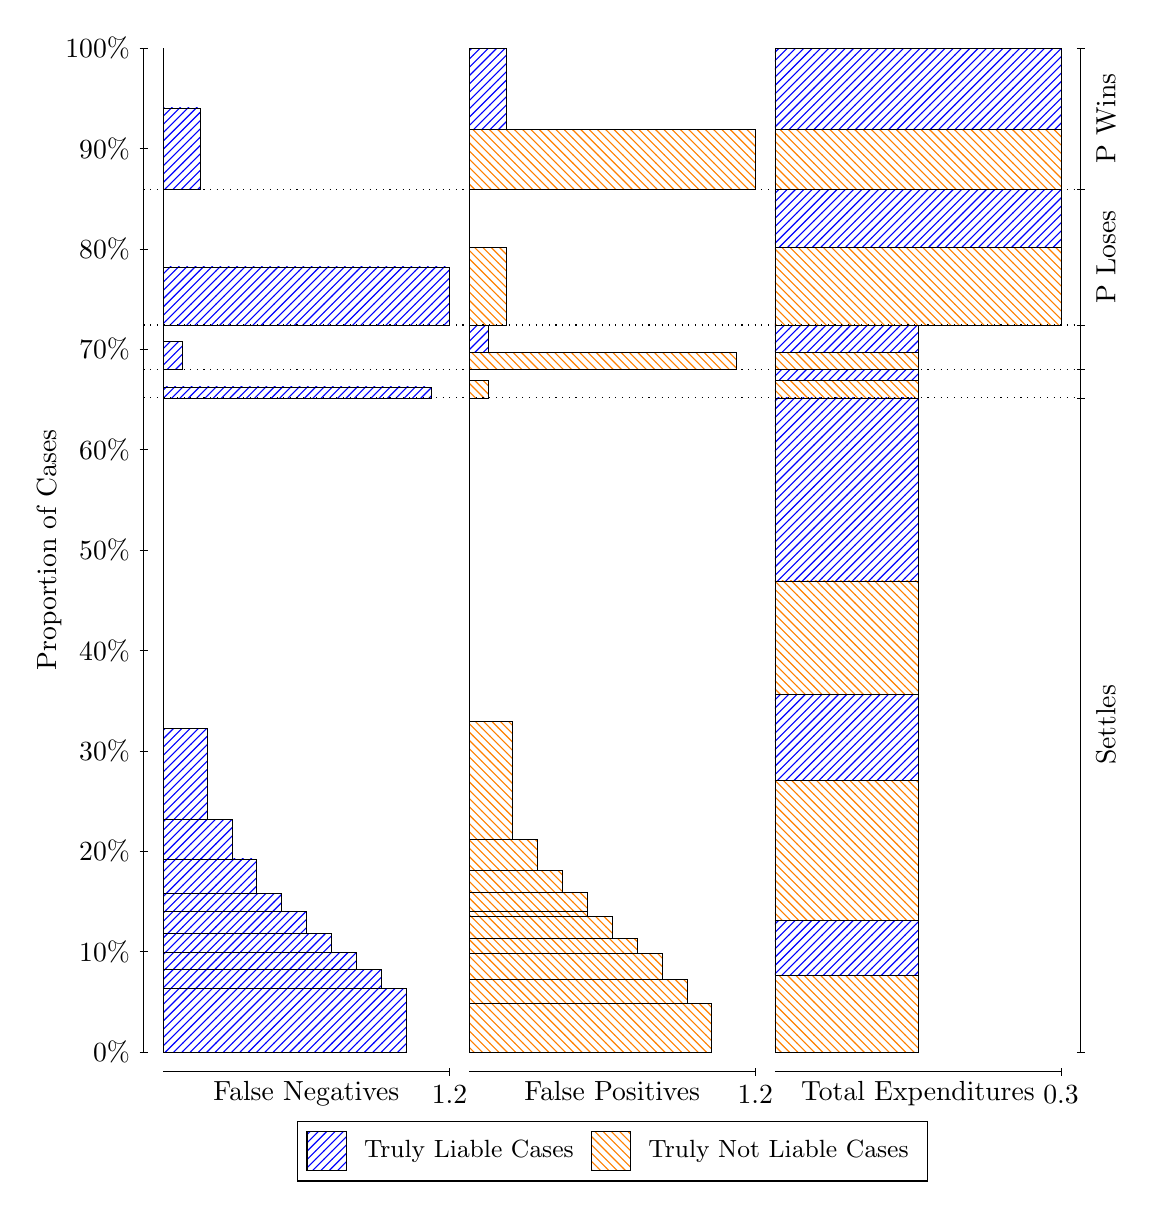
\begin{tikzpicture}
\draw[black, very thin] (1.5,1.75) -- (1.5,14.5);
\node[rotate=90, anchor=center] at (0.3, 8.125) {Proportion of Cases};
\draw[black, very thin] (1.45,1.75) -- (1.55,1.75);
\node[anchor=east] at (1.45, 1.75) {0\%};
\draw[black, very thin] (1.45,3.025) -- (1.55,3.025);
\node[anchor=east] at (1.45, 3.025) {10\%};
\draw[black, very thin] (1.45,4.3) -- (1.55,4.3);
\node[anchor=east] at (1.45, 4.3) {20\%};
\draw[black, very thin] (1.45,5.575) -- (1.55,5.575);
\node[anchor=east] at (1.45, 5.575) {30\%};
\draw[black, very thin] (1.45,6.85) -- (1.55,6.85);
\node[anchor=east] at (1.45, 6.85) {40\%};
\draw[black, very thin] (1.45,8.125) -- (1.55,8.125);
\node[anchor=east] at (1.45, 8.125) {50\%};
\draw[black, very thin] (1.45,9.4) -- (1.55,9.4);
\node[anchor=east] at (1.45, 9.4) {60\%};
\draw[black, very thin] (1.45,10.675) -- (1.55,10.675);
\node[anchor=east] at (1.45, 10.675) {70\%};
\draw[black, very thin] (1.45,11.95) -- (1.55,11.95);
\node[anchor=east] at (1.45, 11.95) {80\%};
\draw[black, very thin] (1.45,13.225) -- (1.55,13.225);
\node[anchor=east] at (1.45, 13.225) {90\%};
\draw[black, very thin] (1.45,14.5) -- (1.55,14.5);
\node[anchor=east] at (1.45, 14.5) {100\%};

\draw[black, very thin] (13.4,1.75) -- (13.4,14.5);
\draw[black, very thin] (13.35,1.75) -- (13.45,1.75);
\node[anchor=west] at (13.35, 1.75) {};
\draw[black, very thin] (13.35,10.057) -- (13.45,10.057);
\node[anchor=west] at (13.35, 10.057) {};
\draw[black, very thin] (13.35,10.422) -- (13.45,10.422);
\node[anchor=west] at (13.35, 10.422) {};
\draw[black, very thin] (13.35,10.982) -- (13.45,10.982);
\node[anchor=west] at (13.35, 10.982) {};
\draw[black, very thin] (13.35,12.707) -- (13.45,12.707);
\node[anchor=west] at (13.35, 12.707) {};
\draw[black, very thin] (13.35,14.5) -- (13.45,14.5);
\node[anchor=west] at (13.35, 14.5) {};

\draw[black, very thin, pattern color=blue, pattern=north east lines] (1.75,1.75) rectangle (4.8304,2.5612);
\draw[black, very thin, pattern color=blue, pattern=north east lines] (1.75,2.5612) rectangle (4.5145,2.8012);
\draw[black, very thin, pattern color=blue, pattern=north east lines] (1.75,2.8012) rectangle (4.1986,3.0145);
\draw[black, very thin, pattern color=blue, pattern=north east lines] (1.75,3.0145) rectangle (3.8826,3.2572);
\draw[black, very thin, pattern color=blue, pattern=north east lines] (1.75,3.2572) rectangle (3.5667,3.5378);
\draw[black, very thin, pattern color=blue, pattern=north east lines] (1.75,3.5378) rectangle (3.2507,3.7635);
\draw[black, very thin, pattern color=blue, pattern=north east lines] (1.75,3.7635) rectangle (2.9348,4.2032);
\draw[black, very thin, pattern color=blue, pattern=north east lines] (1.75,4.2032) rectangle (2.6188,4.7066);
\draw[black, very thin, pattern color=blue, pattern=north east lines] (1.75,4.7066) rectangle (2.3029,5.863);
\draw[black, very thin, pattern color=orange, pattern=north west lines] (1.75,5.863) rectangle (1.75,10.057);
\draw[black, very thin, pattern color=blue, pattern=north east lines] (1.75,10.057) rectangle (5.1464,10.197);
\draw[black, very thin, pattern color=orange, pattern=north west lines] (1.75,10.197) rectangle (1.75,10.422);
\draw[black, very thin, pattern color=blue, pattern=north east lines] (1.75,10.422) rectangle (1.987,10.772);
\draw[black, very thin, pattern color=orange, pattern=north west lines] (1.75,10.772) rectangle (1.75,10.982);
\draw[black, very thin, pattern color=blue, pattern=north east lines] (1.75,10.982) rectangle (5.3833,11.721);
\draw[black, very thin, pattern color=orange, pattern=north west lines] (1.75,11.721) rectangle (1.75,12.707);
\draw[black, very thin, pattern color=blue, pattern=north east lines] (1.75,12.707) rectangle (2.2239,13.74);
\draw[black, very thin, pattern color=orange, pattern=north west lines] (1.75,13.74) rectangle (1.75,14.5);
\draw[black, very thin, pattern color=orange, pattern=north west lines] (5.6333,1.75) rectangle (8.7138,2.365);
\draw[black, very thin, pattern color=orange, pattern=north west lines] (5.6333,2.365) rectangle (8.3978,2.6724);
\draw[black, very thin, pattern color=orange, pattern=north west lines] (5.6333,2.6724) rectangle (8.0819,3.0053);
\draw[black, very thin, pattern color=orange, pattern=north west lines] (5.6333,3.0053) rectangle (7.7659,3.1948);
\draw[black, very thin, pattern color=orange, pattern=north west lines] (5.6333,3.1948) rectangle (7.45,3.4731);
\draw[black, very thin, pattern color=orange, pattern=north west lines] (5.6333,3.4731) rectangle (7.1341,3.5416);
\draw[black, very thin, pattern color=orange, pattern=north west lines] (5.6333,3.5416) rectangle (7.1341,3.7729);
\draw[black, very thin, pattern color=orange, pattern=north west lines] (5.6333,3.7729) rectangle (6.8181,4.0563);
\draw[black, very thin, pattern color=orange, pattern=north west lines] (5.6333,4.0563) rectangle (6.5022,4.4453);
\draw[black, very thin, pattern color=orange, pattern=north west lines] (5.6333,4.4453) rectangle (6.1862,5.9441);
\draw[black, very thin, pattern color=blue, pattern=north east lines] (5.6333,5.9441) rectangle (5.6333,10.057);
\draw[black, very thin, pattern color=orange, pattern=north west lines] (5.6333,10.057) rectangle (5.8703,10.282);
\draw[black, very thin, pattern color=blue, pattern=north east lines] (5.6333,10.282) rectangle (5.6333,10.422);
\draw[black, very thin, pattern color=orange, pattern=north west lines] (5.6333,10.422) rectangle (9.0297,10.632);
\draw[black, very thin, pattern color=blue, pattern=north east lines] (5.6333,10.632) rectangle (5.8703,10.982);
\draw[black, very thin, pattern color=orange, pattern=north west lines] (5.6333,10.982) rectangle (6.1072,11.969);
\draw[black, very thin, pattern color=blue, pattern=north east lines] (5.6333,11.969) rectangle (5.6333,12.707);
\draw[black, very thin, pattern color=orange, pattern=north west lines] (5.6333,12.707) rectangle (9.2667,13.467);
\draw[black, very thin, pattern color=blue, pattern=north east lines] (5.6333,13.467) rectangle (6.1072,14.5);
\draw[black, very thin, pattern color=orange, pattern=north west lines] (9.5167,1.75) rectangle (11.333,2.7222);
\draw[black, very thin, pattern color=blue, pattern=north east lines] (9.5167,2.7222) rectangle (11.333,3.4182);
\draw[black, very thin, pattern color=orange, pattern=north west lines] (9.5167,3.4182) rectangle (11.333,5.1952);
\draw[black, very thin, pattern color=blue, pattern=north east lines] (9.5167,5.1952) rectangle (11.333,6.287);
\draw[black, very thin, pattern color=orange, pattern=north west lines] (9.5167,6.287) rectangle (11.333,7.7319);
\draw[black, very thin, pattern color=blue, pattern=north east lines] (9.5167,7.7319) rectangle (11.333,10.057);
\draw[black, very thin, pattern color=orange, pattern=north west lines] (9.5167,10.057) rectangle (11.333,10.282);
\draw[black, very thin, pattern color=blue, pattern=north east lines] (9.5167,10.282) rectangle (11.333,10.422);
\draw[black, very thin, pattern color=orange, pattern=north west lines] (9.5167,10.422) rectangle (11.333,10.632);
\draw[black, very thin, pattern color=blue, pattern=north east lines] (9.5167,10.632) rectangle (11.333,10.982);
\draw[black, very thin, pattern color=orange, pattern=north west lines] (9.5167,10.982) rectangle (13.15,11.969);
\draw[black, very thin, pattern color=blue, pattern=north east lines] (9.5167,11.969) rectangle (13.15,12.707);
\draw[black, very thin, pattern color=orange, pattern=north west lines] (9.5167,12.707) rectangle (13.15,13.467);
\draw[black, very thin, pattern color=blue, pattern=north east lines] (9.5167,13.467) rectangle (13.15,14.5);
\draw[black, dotted] (1.5,10.057) -- (13.4,10.057);
\draw[black, dotted] (1.5,10.422) -- (13.4,10.422);
\draw[black, dotted] (1.5,10.982) -- (13.4,10.982);
\draw[black, dotted] (1.5,12.707) -- (13.4,12.707);
\draw[black, very thin] (1.75,1.5) -- (5.3833,1.5);
\node[anchor=north] at (3.5667, 1.5) {False Negatives};
\draw[black, very thin] (5.3833,1.45) -- (5.3833,1.55);
\node[anchor=north] at (5.3833, 1.45) {1.2};

\draw[black, very thin] (5.6333,1.5) -- (9.2667,1.5);
\node[anchor=north] at (7.45, 1.5) {False Positives};
\draw[black, very thin] (9.2667,1.45) -- (9.2667,1.55);
\node[anchor=north] at (9.2667, 1.45) {1.2};

\draw[black, very thin] (9.5167,1.5) -- (13.15,1.5);
\node[anchor=north] at (11.333, 1.5) {Total Expenditures};
\draw[black, very thin] (13.15,1.45) -- (13.15,1.55);
\node[anchor=north] at (13.15, 1.45) {0.3};

\node[black, centered, rotate=90] at (13.72, 5.9035) {Settles};


\node[black, centered, rotate=90] at (13.72, 11.845) {P Loses};
\node[black, centered, rotate=90] at (13.72, 13.604) {P Wins};

\draw (7.449999999999999,1.5) node[draw=none] (baseCoordinate) {};
\begin{scope}[align=center]
        \matrix[scale=0.5, draw=black, below=0.5cm of baseCoordinate, nodes={draw}, column sep=0.1cm]{
            \node[rectangle, draw, minimum width=0.5cm, minimum height=0.5cm, pattern=north east lines, pattern color=blue] {}; &
            \node[draw=none, font=\small] (B) {Truly Liable Cases}; &
            \node[rectangle, draw, minimum width=0.5cm, minimum height=0.5cm, pattern=north west lines, pattern color=orange] {}; &
            \node[draw=none, font=\small] (B) {Truly Not Liable Cases}; \\
            };
\end{scope}

\end{tikzpicture}
\end{document}